Por normal general cuando se habla de programación web en el lado del cliente, se tiende a pensar
de forma inmediata en Javascript, y en general, este razonamiento es indudablemente válido. 
Pero dado que SIMDE es una aplicación fuertemente orientada a objetos y con una gran base de código, 
se han valorado múltiples alternativas con el objetivo de agilizar la realización de este proyecto.

\subsection{Coffescript}

Coffescript es un pequeño lenguaje que se compila en Javascript, su objetivo era mejorar la legibilidad 
y concisión de Javascript añadiendo varios \textit{syntactic sugars} inspirados en otros lenguajes como
\textit{Ruby} o \textit{Python}. \cite{Coffescript}

\bigskip
Coffescript es un lenguaje con un largo recorrido, apareciendo a finales del año 2009. Y tiene soporte por
parte de \textit{Ruby on Rails} y \textit{Play framework}. \cite{CoffescriptWiki}

\bigskip 
Coffescript podría ser la opción ideal para agilizar le desarrollo debido a la similitud de sintaxis con 
Ruby.

\begin{lstlisting}
class Animal
  constructor: (@name) ->

  alive: ->
    false

class Parrot extends Animal
  constructor: ->
    super("Parrot")

  dead: ->
    not @alive()
\end{lstlisting}

\bigskip
Sin embargo, la opción de Coffescript ha sido desestimada en gran medida por su decreciente popularidad
y la poca certeza del futuro que tomará el lenguaje.

\subsection{Dart}

Dart es un lenguaje de código abierto desarrollado por Google que permite desarrollador aplicaciones web, móvil, 
de servidor y también se puede utilizar en el \textit{Internet of Things}. \cite{Dart}

\bigskip
Se ha considerado en el desarrollo de esta aplicación porque es un lenguaje orientado a objetos que utiliza una 
sintaxis similar a C\#. Además, aunque Google Chrome tiene una máquina virtual nativa para este lenguaje, es posible
transpilar el código a Javascript para los navegadores que no tiene este soporte nativo.

\bigskip
Tras razonar detenidamente, ha pesar de lo atractivo del lenguaje, Dart ha quedado descartado por 
una razón de peso y es que se trata de un lenguaje totalmente diferente y su uso es mayoritariamente
por parte de Google.

\subsection{Typescript}

Typescript es un lenguaje libre y de código abierto desarrollado por Microsoft que actúa como un superconjunto
de Javascript, es decir incorpora los distintos estándares: ECMA5, ECMA6, ECMA7... Y además, como característica
destacable, añade comprobación de tipos en tiempo de compilación. \cite{Typescript}

\bigskip
Este tipado no se refleja en el código final, de hecho una interfaz, por ejemplo,
añade 0 sobrecarga en el código final. Pero si que es interesante por las capacidades de
autocompletado (a través de Microsoft Intellisense)  que añade.

\begin{figure}[!th]
\begin{center}
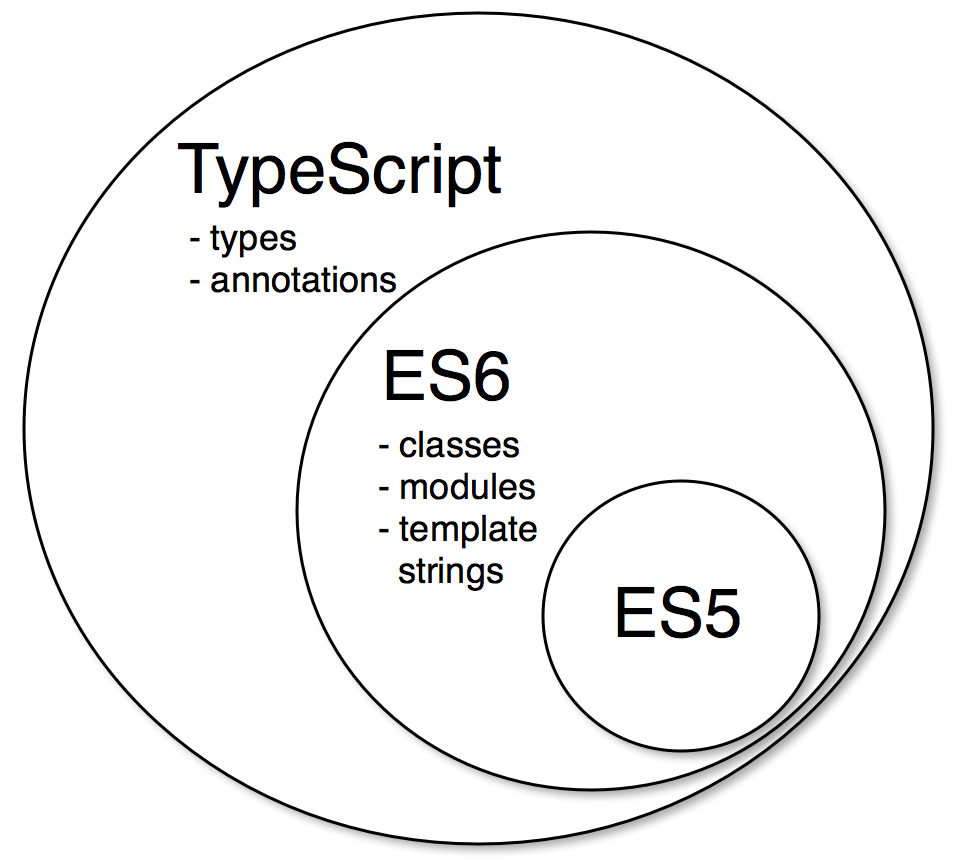
\includegraphics[width=0.5\textwidth]{images/cap4/typescript.eps}
\caption{Typescript como superconjunto de Javascript}
\label{fig:Typescript como superconjunto de Javascript}
\end{center}
\end{figure}

\bigskip
Al final, en este proyecto Typescript ha sido la tecnología ganadora, y existen múltiples
razones:

\begin{enumerate}

\item Typescript tiene bastante apoyo por parte de la comunidad y por parte de la propia Microsoft.
La documentación es extensa y efectiva.

\item Typescript está alineada en cierta forma con el futuro de Javascript. Microsoft es uno de los 
muchos que forman parate del concenso de estándar de ECMASCRIPT.

\item Typescript no me limita en la posibilidad de usar javascript, todo código javascript es código
Typescript válido.

\item Por último y no menos importante: Tengo cierta experiencia con Typescript.
\end{enumerate}

